\chapter{Página de Internet}\label{chap:webPage}

	Como se comentó en el capítulo de introducción una gran ventaja del lenguaje java es su capacidad para crear páginas de internet. En el presente trabajo se creó una página de internet cuyo objetivo es exponer las funciones principales de la librería materia.

	La página se encuentra en la dirección web: \url{chimicae-materia.rhcloud.com}, se recomienda utilizar un navegador moderno como google chrome.

	El presente capítulo trata sobre como utilizar la página para:

	\begin{itemize}
		\item{Crear}
			\begin{itemize}
				\item{Substancias} Sección \ref{sec:webSubstanceCreator}
				\item{Mezclas} Sección \ref{sec:webMixtureCreator}
			\end{itemize}
		\item{Gráficas}
			\begin{itemize}
				\item \nameref{subsec:pvt}
				\item \nameref{subsec:zpt}
				\item \nameref{subsec:fpt}
				\item \nameref{subsec:tep}
				\item \nameref{subsec:tsp}
				\item \nameref{subsec:tgp}
				\item \nameref{subsec:tpv}
			\end{itemize}
		\item{Estimación de parámetros}
			\begin{itemize}
				\item Expresión de $\alpha$
				\item Regla de Mezclado
			\end{itemize}
	\end{itemize}

\section{Selección de compuestos puros}\label{sec:webCompounds}

	La página de internet dispone de la base de datos ChemSep v6.96 derechos de autor  Harry Kooijman y Ross Taylor (2013) bajo la licencia `Artistic License': \url{ http://www.perlfoundation.org/artistic_license_2_0}.

	Primero se deben cargar los compuestos puros en la sección `Creación' - `Compuesto Puro'. Para buscar compuestos se debe escribir el nombre en inglés del compuesto deseado en el recuadro de texto al lado de la etiqueta `Buscar'. Al dar click en el boton buscar la página buscará coincidencias entre el nombre escrito y los nombres de la base de datos. Los compuestos que muestren coincidencia con el texto escrito se mostrarán en una lista debajo del recuadro.

	Para agregar un compuesto de la lista basta con dar click en el boton `Agregar' junto al nombre del compuesto. En la tabla a la derecha de la página se muestran los compuestos agregados. Ver la figura \ref{fig:pureCompounds}.

	\begin{figure}[!h]
		\centering
		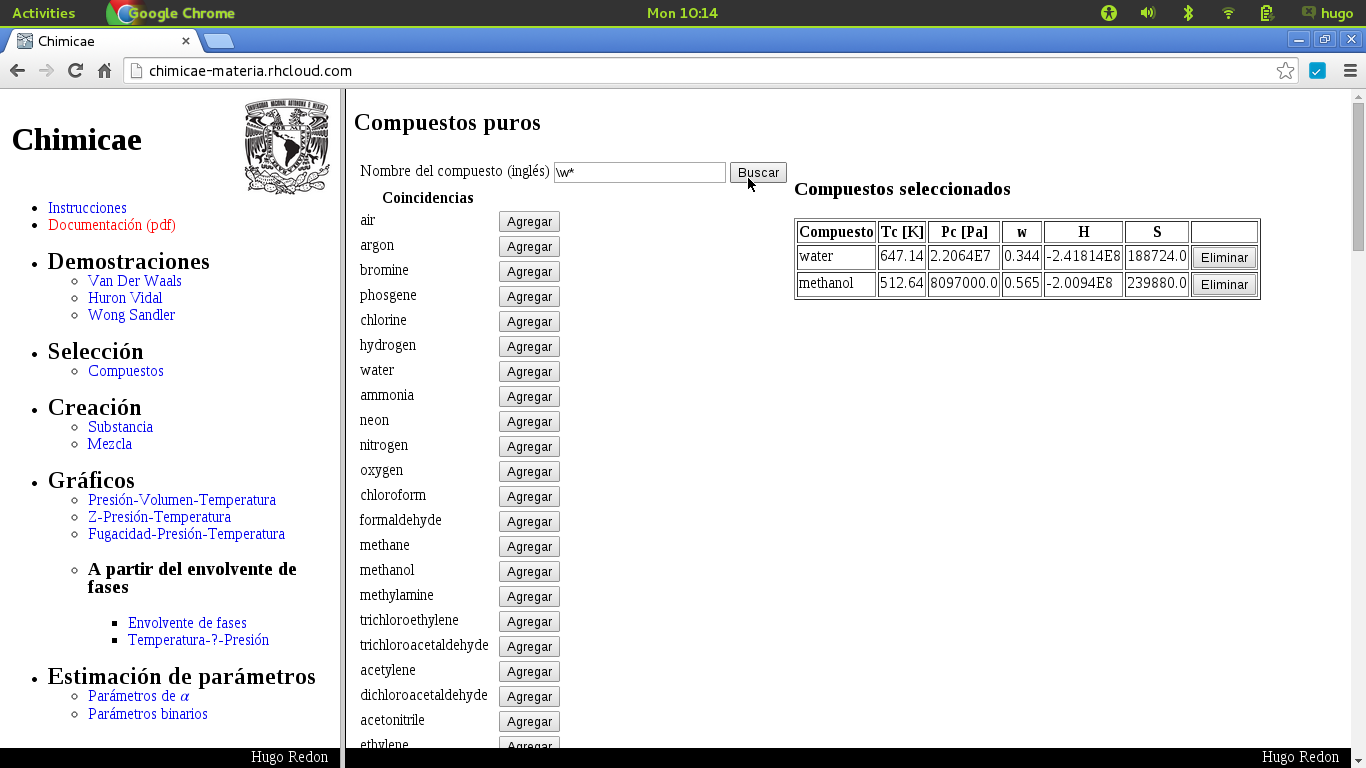
\includegraphics[scale=0.34]{pureCompounds.png}
		\caption{Formulario para seleccionar y cargar compuestos puros en la página de internet}
		\label{fig:pureCompounds}
	\end{figure}

\section{Creación de substancias}\label{sec:webSubstanceCreator}
	
	En la sección `Creación' - `Substancia' se permite crear materia de un solo compuesto, para después utilizarse en las secciones de graficación y estimación de parámetros de la expresión de $\alpha$.

	Esta sección permite elegir la ecuación cúbica, la expresión de $\alpha$, el compuesto y la fase homogéna con la cual se creará la substancia. Al final de la sección el botón `Aceptar' creará la Substancia y mostrará el resultado de la creación.

	La figura \ref{fig:substanceCreator} muestra la interfaz de usuario para la creación de substancias. La figura \ref{fig:substanceProperties} muestra las propiedades de la substancia creada.

	\begin{figure}[!h]
		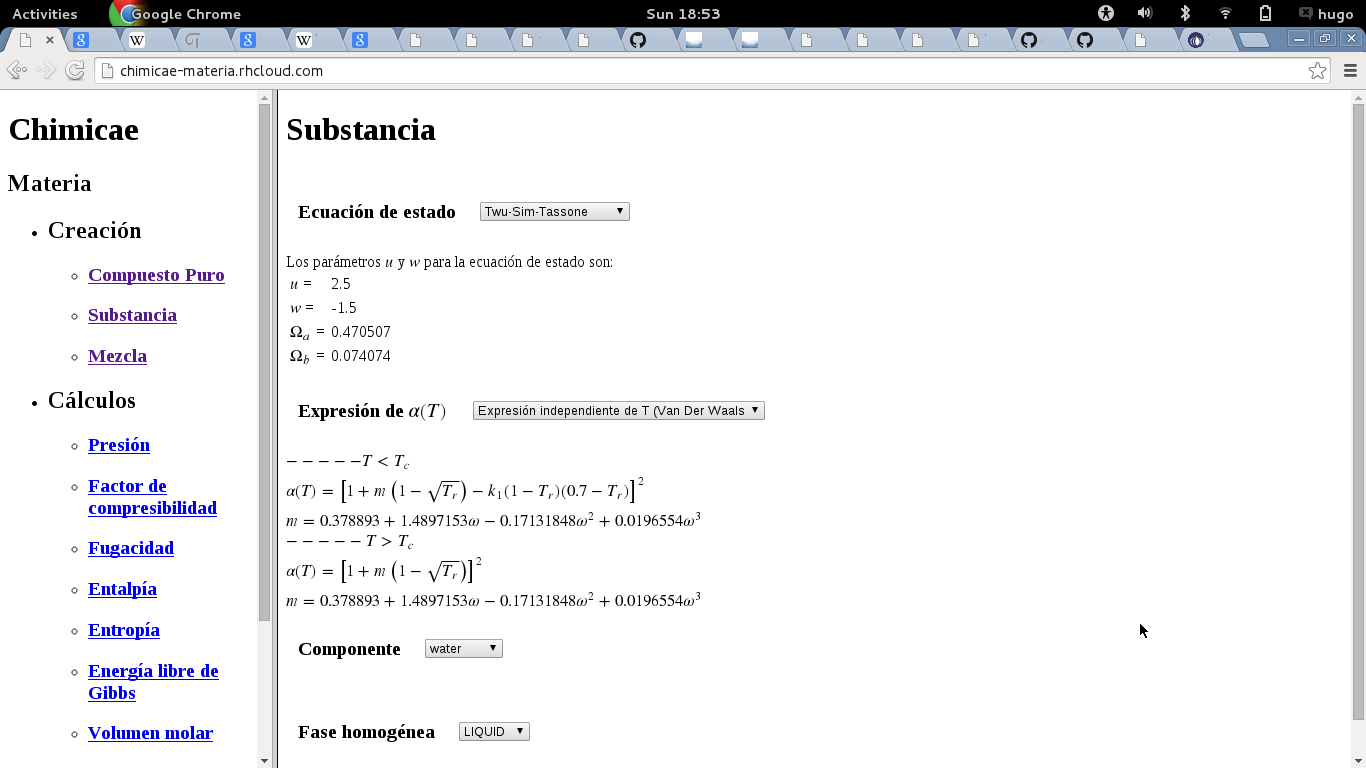
\includegraphics[scale=0.3]{substanceCreator.png}
		\caption{Formulario para crear substancias en la página de internet}
		\label{fig:substanceCreator}
	\end{figure}

	\begin{figure}[!h]
		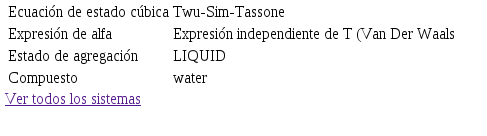
\includegraphics[scale=0.3]{substanceProperties.png}
		\caption{Página que muestra las propiedades de la substancia recien creada}
		\label{fig:substanceProperties}
	\end{figure}

\section{Creación de Mezclas}\label{sec:webMixtureCreator}

	En la sección `Creación' - `Mezcla' se permite crear materia con multiples compuestos, solo aquellas mezclas que contengan dos compuestos estarán disponibles en la sección de estimación de parámetros binarios \ref{sec:webBinaryOptim}.

	El formulario permite elegir la ecuación cúbica, la fase ,la regla de mezclado, permite elegir cada compuesto, definir su expresión de $\alpha$ y su fración molar. Ver figura \ref{fig:webMixCreator}.

	\begin{figure}[!h]
		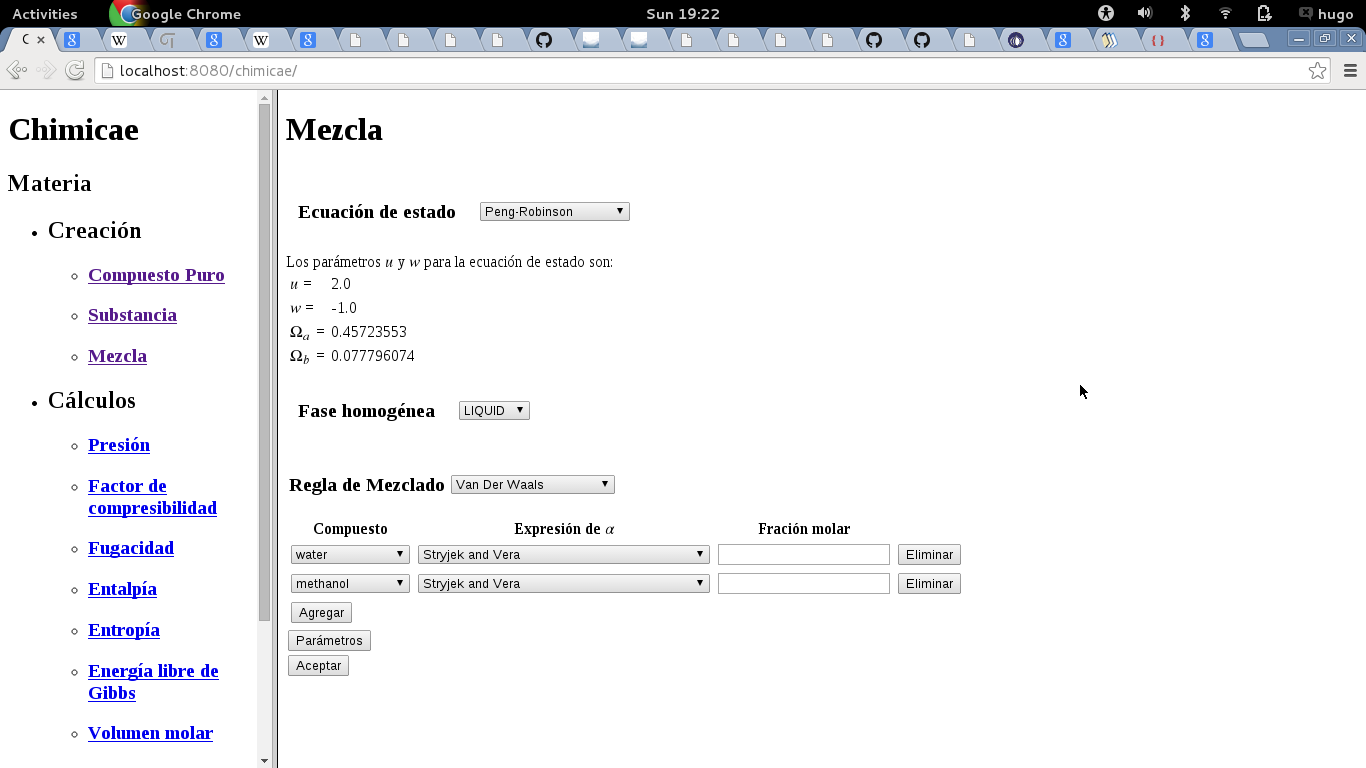
\includegraphics[scale=0.3]{mixtureCreator.png}
		\caption{Formulario para la creación de mezclas}
		\label{fig:webMixCreator}
	\end{figure}

	El botón con la etiqueta `Parámetros' permite definir los parámetros binarios para la regla de mezclado seleccionada. Finalmente el botón `Aceptar' construye la mezcla y la pone a disposición para las siguientes secciones.

\section{Gráficos}

	Las secciónes de gráficos dividen el recuadro derecho de forma horizontal, en la parte superior se localizan los controles de las gráficas, y en la parte inferior la gŕafica tridimensional.

	En esta sección estan disponibles las substancias y mezclas creadas anteriormente, basta con dar click en la caja tipo `combobox' y selecciónar el sistema, esto es igual para todas las gráficas de la sección.

	En algunas gráficas se muestran los resultados de la fase líquida y vapor sin importar la fase seleccionada en el momento de la creación del sistema.

	\subsection{Presión-Volumen-Temperatura}\label{subsec:pvt}
		En este tipo de gráfica no se involucra la fase del sistema. 

		La sección de controles permite elegir el rango del volumen molar y el rango de temperatura.
		
		El propósito de la figura \ref{fig:press} es observar los puntos de inflexión característicos de las ecuaciones cúbicas, en el caso que ellos se encuentren dentro del dominio seleccionado.

		\begin{figure}[!h]
			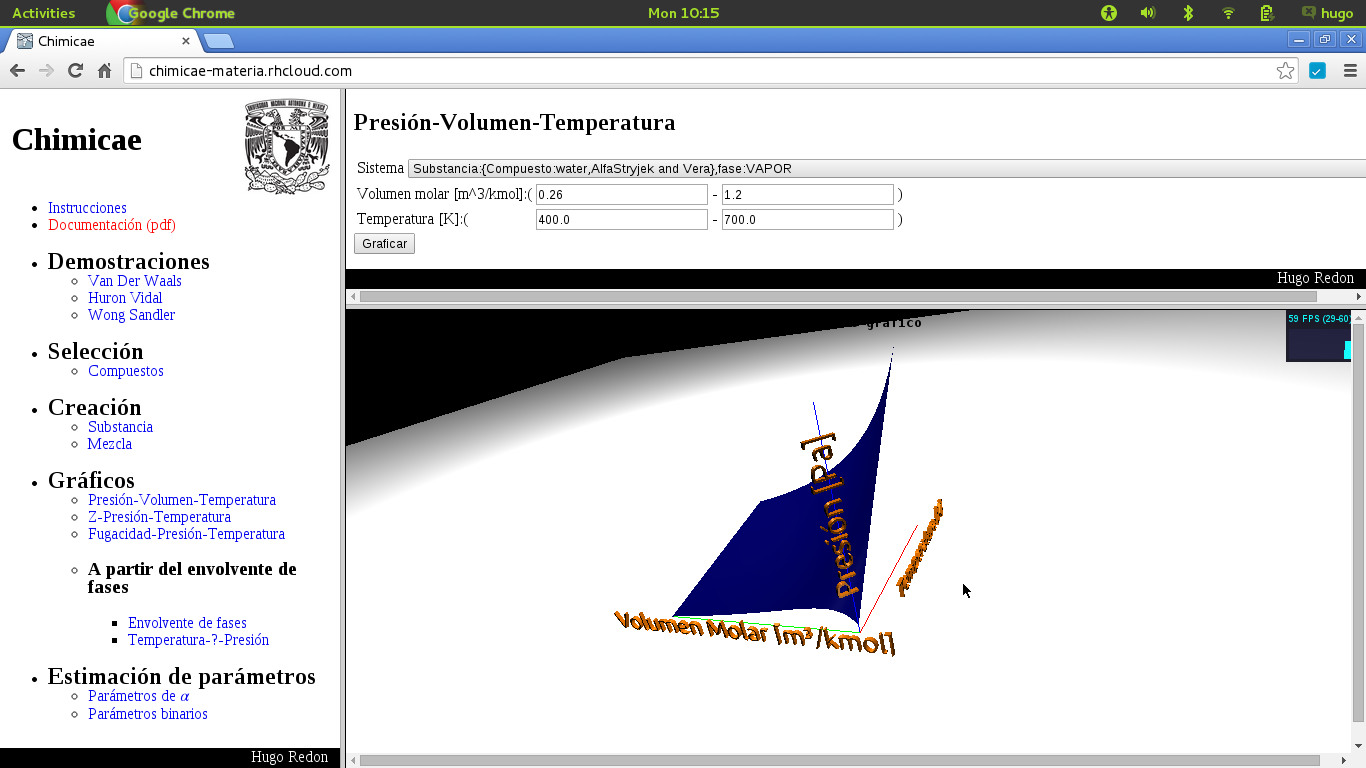
\includegraphics[scale=0.3]{waterPressurePlot.png}
			\caption{Gráfica de presión-volumen-temperatura para el agua con la ecuación de estado de Peng-Robinson y la expresion de $\alpha$ de Stryjek and Vera que esta cargada por default. El rango de volumen: $0.26-1.2 [\frac{m^3}{kmol}]$ y temperatura:$400-700[K]$ }
			\label{fig:press}
		\end{figure}
	\subsection{Z-Presión-Temperatura}\label{subsec:zpt}
		Usualmente las gráficas del factor de compresibilidad se crean en dos dimensiones mostrando diferentes temperaturas en el mismo plano y no es posible ver efecto que se tiene a altas temperaturas y presiones.

		Esta gráfica depende de la fase seleccionada para el sistema.

		Semejante a la sección anterior se debe determinar un rango de presión y temperatura. La figura \ref{fig:zplot} muestra el efecto en tercera dimensión.
		\begin{figure}[!h]
			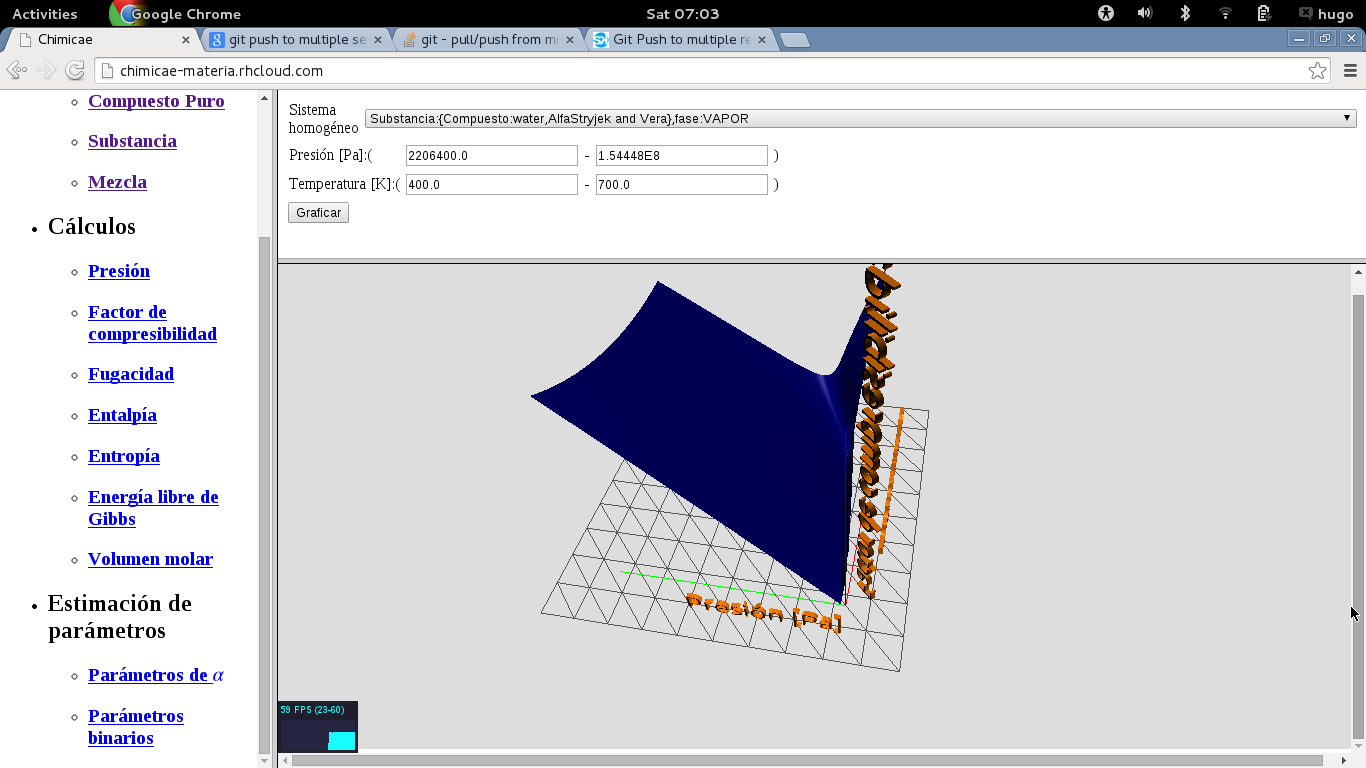
\includegraphics[scale=0.3]{waterZPlot.png}
			\caption{Gŕafica de z(Factor de compresibilidad)-Presión-Temperatura para el agua con la ecuación de estado de Peng-Robinson y la expresiónde $\alpha$ Stryjek and Vera.}
			\label{fig:zplot}
		\end{figure}
	\subsection{Fugacidad-Presión-Temperatura}\label{subsec:fpt}

		En esta gráfica se dibujan las curvas de fugacidad para las dos fases, para el líquido (rojo) y el vapor (azul).

		El objetivo de la gráfica es observar el equilibrio líquido-vapor en la línea de intersección de los planos. Ver la figura \ref{fig:fugplot}.

		La línea de equilibrio (Intersección de los planos) puede aparecer o no, dependiendo del dominio elegido.

		\begin{figure}[!h]
			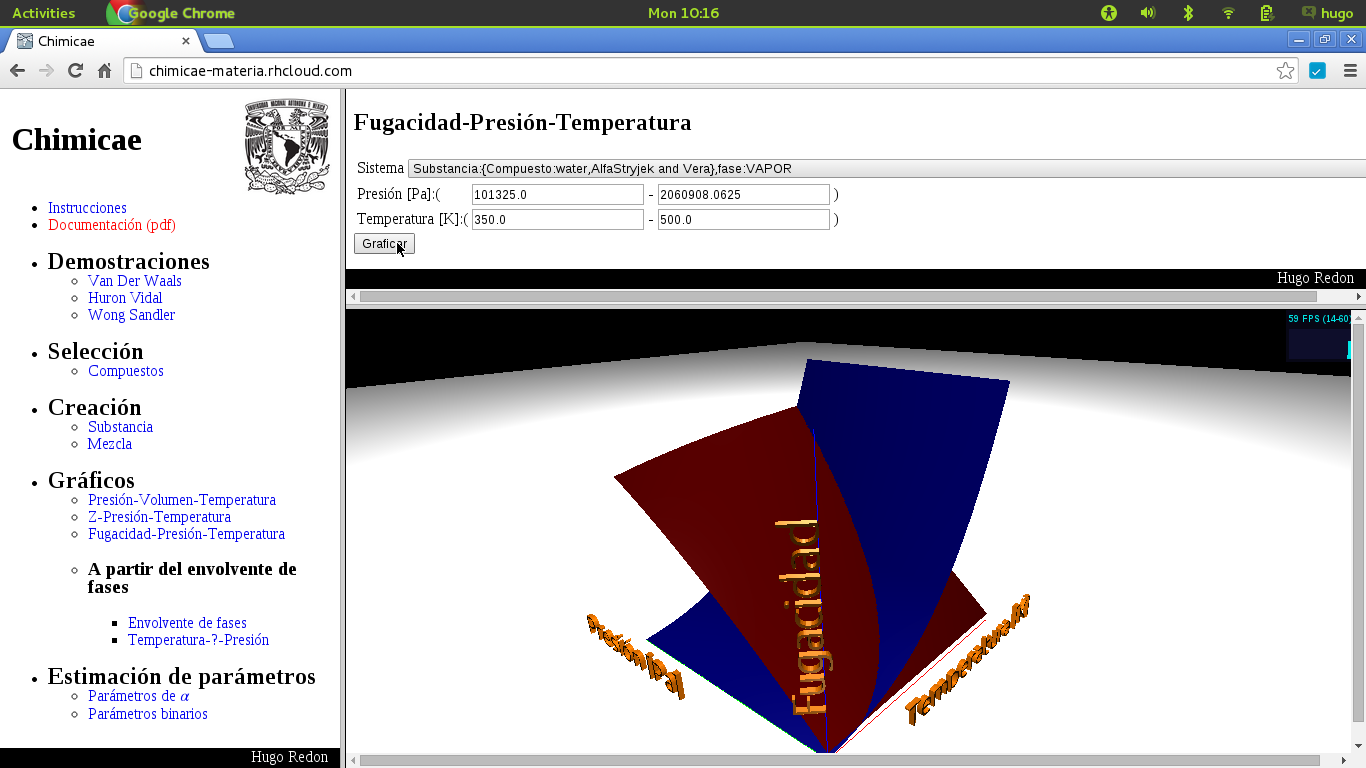
\includegraphics[scale=0.3]{waterFugacityPlot.png}
			\caption{Gŕafica de Fugacidad-Presión-Temperatura para el agua con la ecuación de estado de Peng-Robinson y la expresión de $\alpha$ stryjek y Vera}
			\label{fig:fugplot}
		\end{figure}
	\subsection{Temperatura-Entalpía-Presión}\label{subsec:tep}

		En esta y las siguientes gŕaficas se dibujan dos tipos de regiones, la región de dos fases que se identifica con un color rojo y la región de una fase que se identifica con un color azul.

		En estas gráfica no se debe determinar el rango, ya que este se calcula con los puntos críticos y la diferencia de propiedades en las regiones de dos fases. 

		Podemos ver la forma de la gráfica en la figura \ref{fig:hplot}.

		\begin{figure}[!h]
			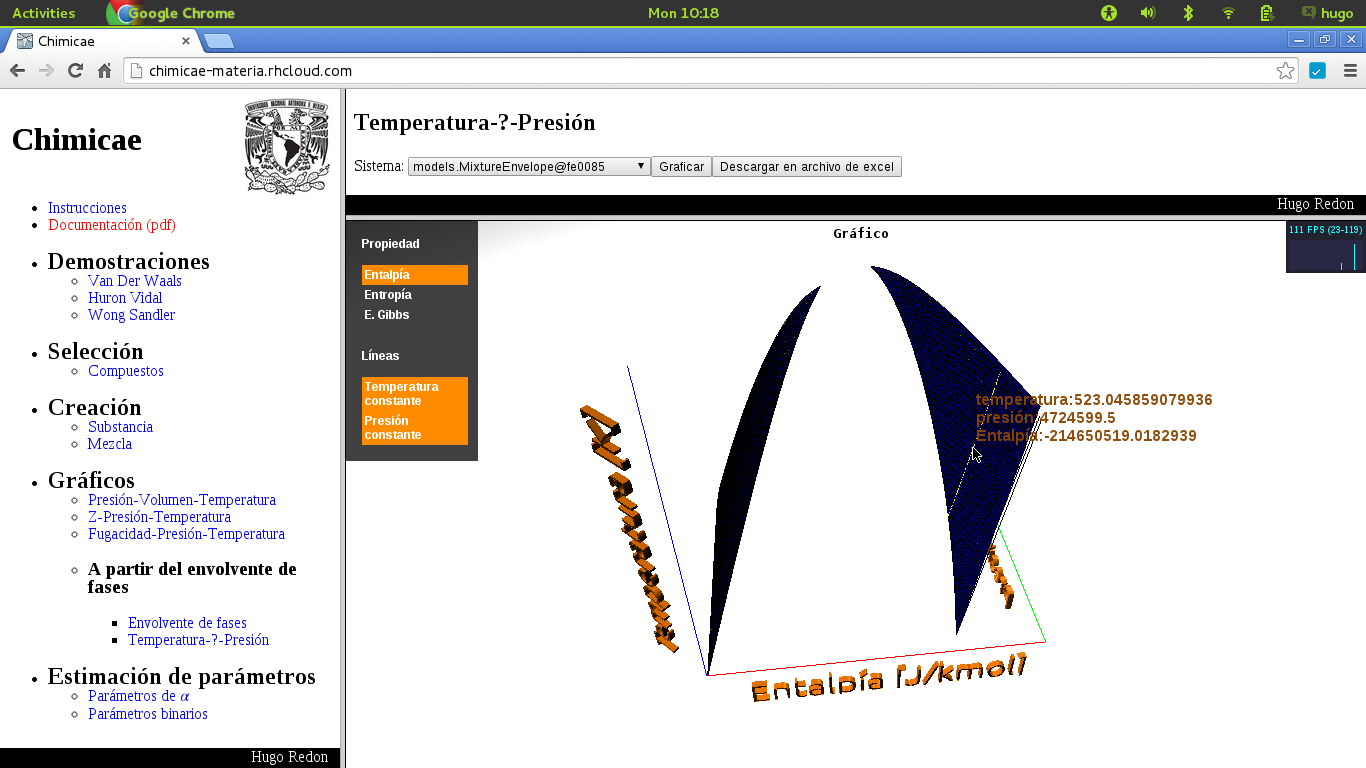
\includegraphics[scale=0.3]{waterEnthalpyPlot.png}
			\caption{Gráfica de Temperatura-Entalpía-Presión para el agua con la ecuación de estado de Peng-Robinson y la expresión de $\alpha$ stryjek y Vera}
			\label{fig:hplot}
		\end{figure}
	\subsection{Temperatura-Entropía-Presión}\label{subsec:tsp}	
		\begin{figure}[H]
			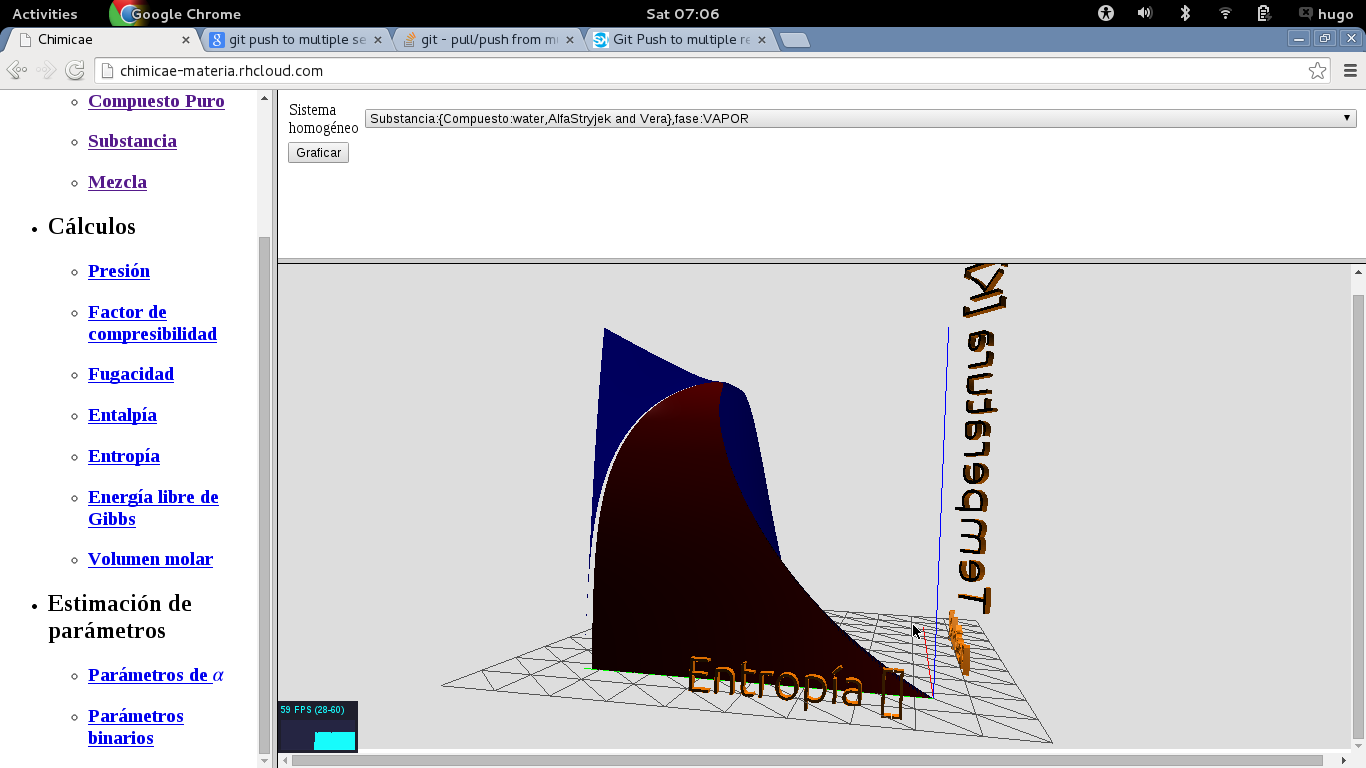
\includegraphics[scale=0.3]{waterEntropyPlot.png}
			\caption{Gráfica de Temperatura-Entropía-Presión para el agua con la ecuación de estado de Peng-Robinson y la expresión de $\alpha$ Stryjek y Vera}
			\label{fig:splot}
		\end{figure}
	\subsection{Temperatura-Gibbs-Presión}\label{subsec:tgp}
		\begin{figure}[H]
			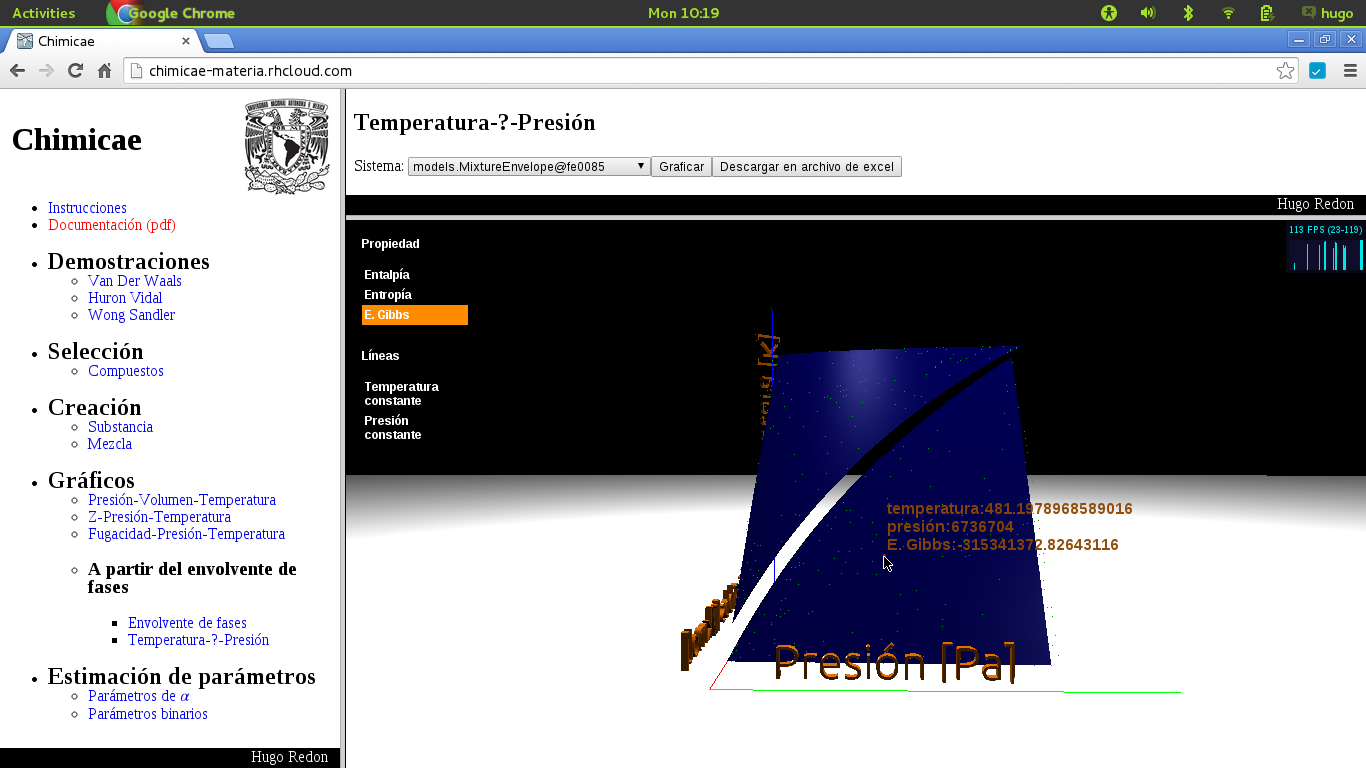
\includegraphics[scale=0.3]{waterEGPlot.png}
			\caption{Gráfica de Temperatura-(Energía libre de Gibbs)-Presión para el agua con la ecuación de estado de Peng-Robinson y la expresión de $\alpha$ de Stryjek y Vera}
			\label{gplot}
		\end{figure}
	\subsection{Temperatura-Presión-Volumen}\label{subsec:tpv}
		\begin{figure}[H]
			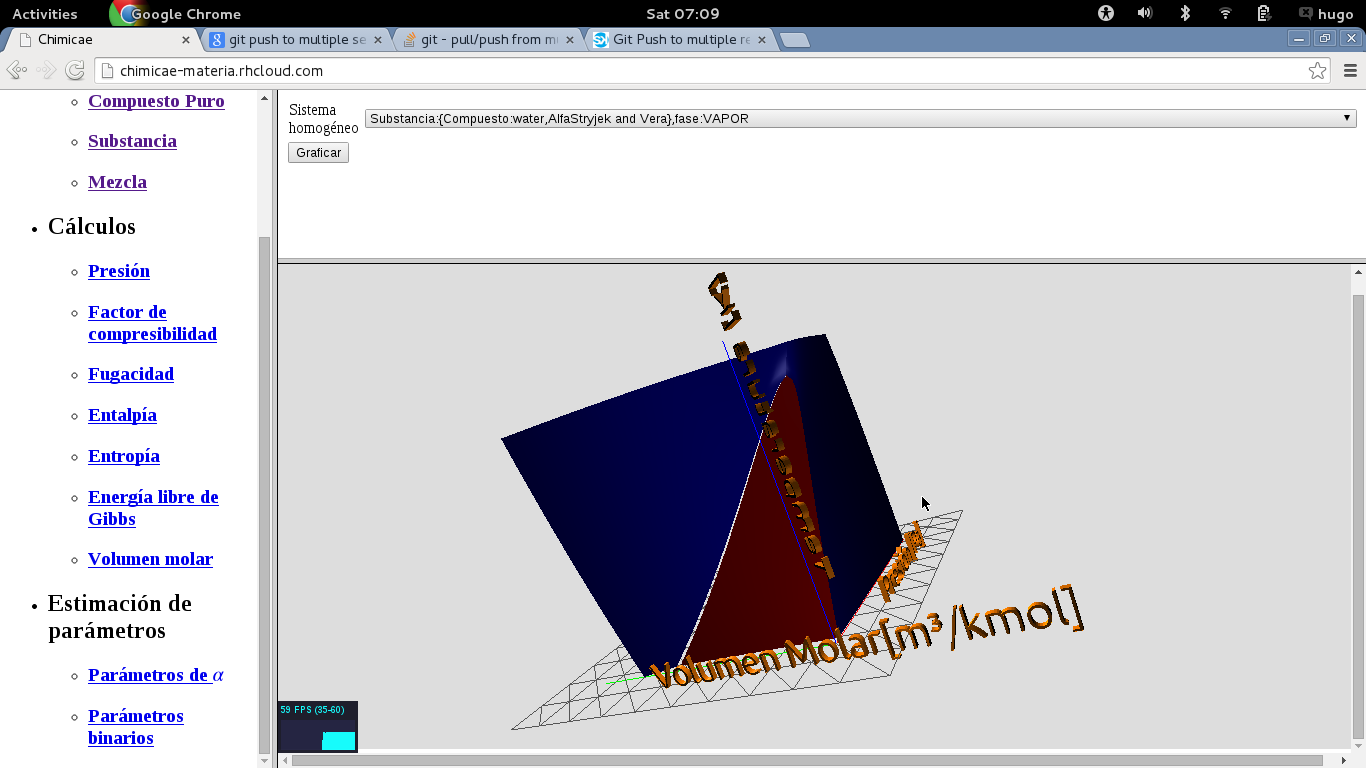
\includegraphics[scale=0.3]{waterVolumePlot.png}
			\caption{Gráfica de Temperatura-Presión-Volumen molar para el agua con la ecuación de estado de Peng-Robinson y la expresión de $\alpha$ de Stryjek y Vera}
			\label{vplot}
		\end{figure}
	
	
\section{Estimación de parámetros de $\alpha$}\label{sec:webAlphaOptim}
	En la sección de `Estimación de parámetros' - `Parámetros de $\alpha$' pódemos seleccionar una de las substancias creadas y estimar sus parámetros con una serie de datos generados a través de la ecuación \ref{eq:101vaporpressure} que nos proporciona la base de datos Chemsep.

	En la sección se muestra una gráfica que compara el modelo con los datos generados, una gráfica que muestra el error relativo, y finalmente una gráfica que muestra la historia de convergencia de la estimación de los parámetros.

	Una imagen del formulario se presenta en la figura \ref{fig:alphaOptim}

\begin{figure}[H]
	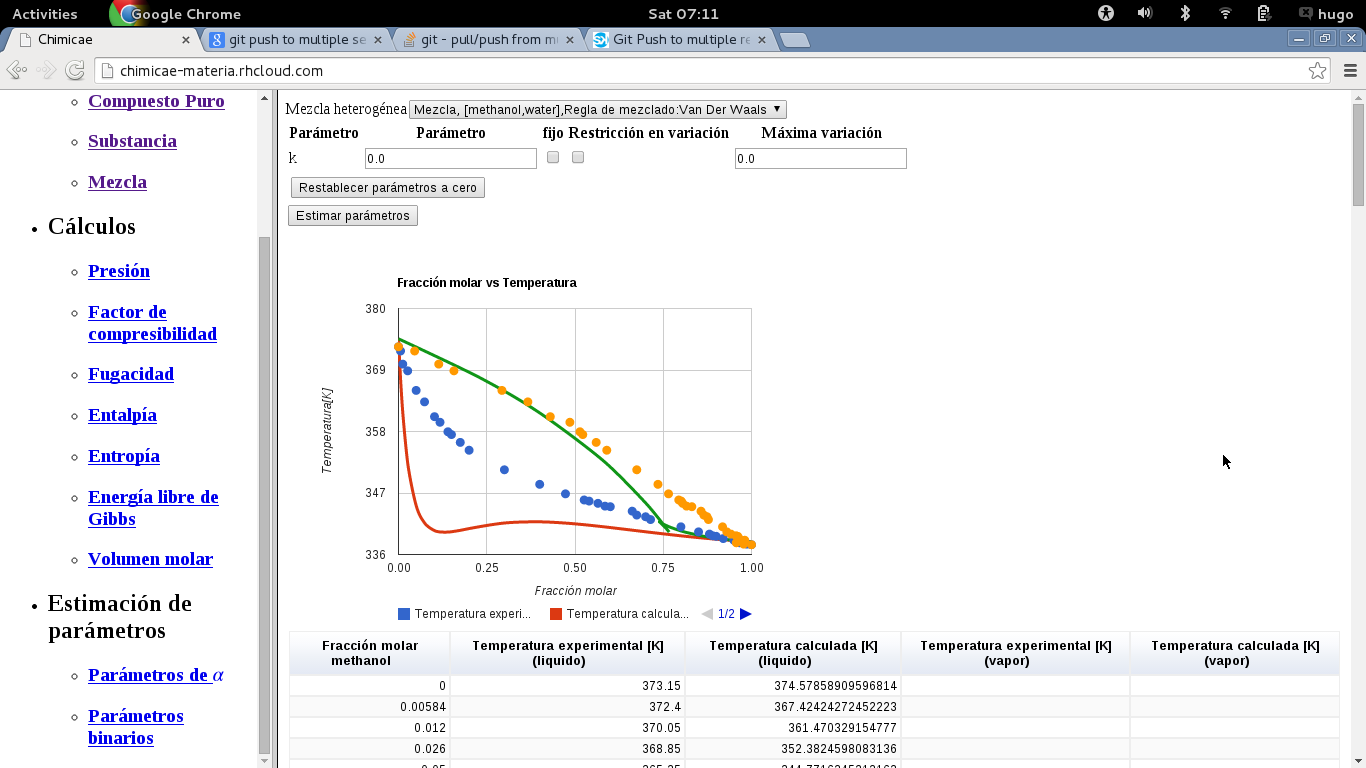
\includegraphics[scale=0.3]{waterMethanolBinaryOptPlot.png}
	\caption{Formulario para la estimación de parámetros de la expresión de $\alpha$}
	\label{fig:alphaOptim}
\end{figure}


\section{Estimación de parámetros binarios de las reglas de mezclado}\label{sec:webBinaryOptim}
	En la sección de `Estimación de parámetros' - `Parámetros binarios' podemos seleccionar una de las mezclas creadas previamente y estimar los parámetros de la regla de mezclado con datos que deberán ser agregados previamente a la página de internet.

	De manera semejante a la sección anterior, en la página se realiza una comparación de los datos experimentales con el modelo, se muestra una gráfica del error relativo y la historia de la convergencia.

	Una imagen del formulario se presenta en la figura \ref{fig:binaryOptim}
\begin{figure}[H]
	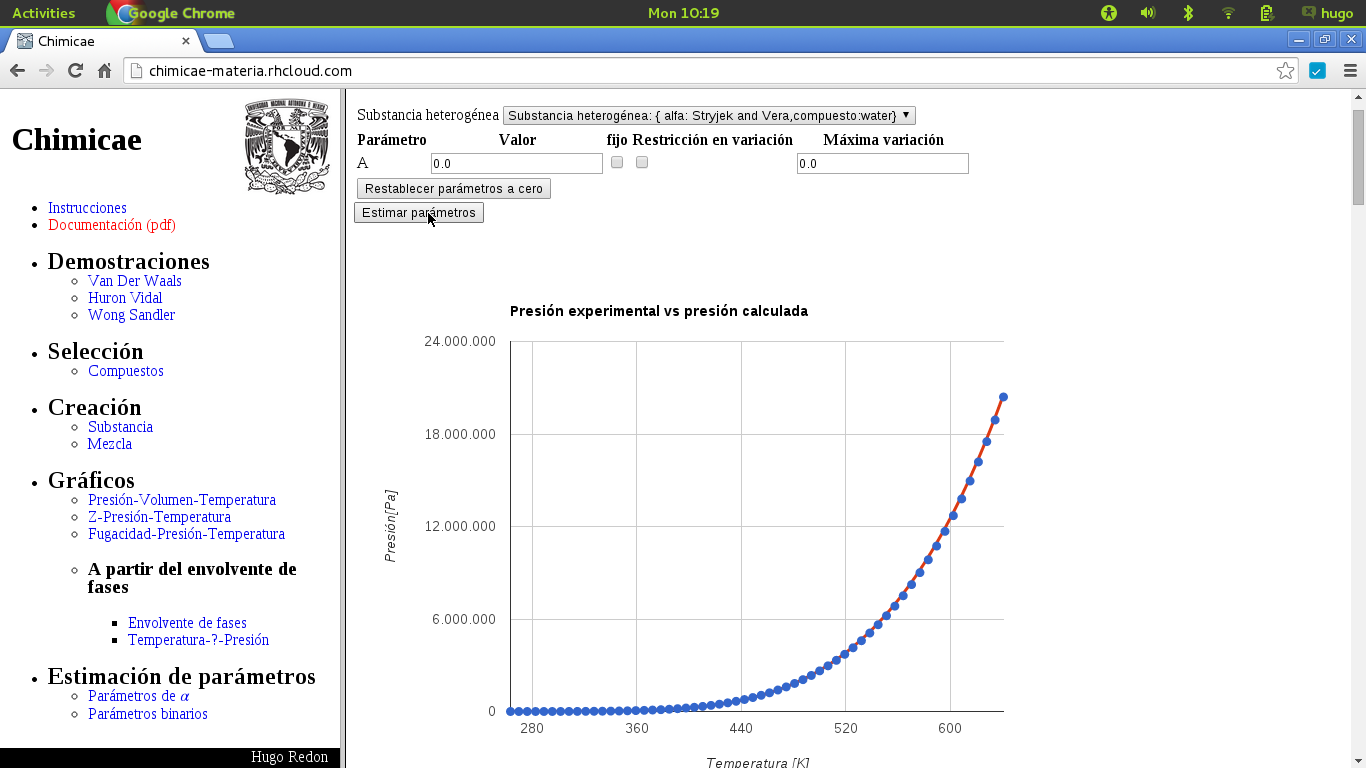
\includegraphics[scale=0.3]{waterAlphaOptPlot.png}
	\caption{Formulario para la estimación de parámetros de la regla de mezclado de Van Der Waals}
	\label{fig:binaryOptim}
\end{figure}
